\documentclass[level=2,teacher]{kidscode}
% Let lines with long code words stretch a little instead of running into the margin.
\setlength{\emergencystretch}{3em}
\newcommand{\bx}{$\square$}
\begin{document}
\kctitle{Project Teacher Guide}{Running the final project: milestones, unblocking, rubric, the Star Catcher reference solution and the Family Arcade showcase}

\setcounter{tocdepth}{1}
\tableofcontents

\section{1. The project at a glance}
Each child (or pair) builds \textbf{either} an arcade game with keys, a timer and a score,
\textbf{or} a generative art studio that saves and loads designs. Every project must use the six
\enquote{must-haves}: functions with parameters and return values, a list, a dictionary, a
\texttt{while} loop or game loop with \texttt{ontimer}, a file, and at least three pytest tests of
their own functions. Goals: L2.G3, G4, G5, G6, G7 and especially \textbf{L2.G8} (plan, work in a team,
act on feedback).

{\small
\renewcommand{\arraystretch}{1.3}
\begin{longtable}{@{}>{\bfseries}p{1.6cm}>{\raggedright\arraybackslash}p{4.4cm}>{\raggedright\arraybackslash}p{8.6cm}@{}}
\toprule
Session & Milestone & What happens \\ \midrule\endhead
Week 9 (last 15 min) & Kickoff, start M1 & Hand out the brief, show Star Catcher for 3 minutes, children choose an option and an idea. M1 pages go home as homework. \\
Week 10 & M1 check, then M2 & First 10 minutes: check each pitch (see 3.1). Paper prototype, then build the core loop from the starter template. \\
Week 11 & M3 then M4 & First half: list, dictionary, file, three tests. Second half: playtest swap, fix one thing, accessibility check. \\
Week 12 & Showcase & Exit assessment (20 min), then the Family Arcade (40 min). \\
\bottomrule
\end{longtable}}

\begin{materials}
  \item Print: the Project Brief (one per child) in week 9; feedback cards (section 7) in week 11 and 12.
  \item On each Mac: the folder \texttt{2-intermediate/project/starter/} (templates, \texttt{my\_tests.py},
        \texttt{README.md}). Each child copies it into their own project folder (the README explains how).
  \item For you: 10 minutes before week 9, play Star Catcher yourself (section 5) so you can demo it.
  \item pytest installed on every Mac (Teacher Guide, section 4.2).
\end{materials}

%% ====================================================================
\section{2. Pairs or solo?}
Both are fine. Pairs build bigger, more fun projects and practise L2.G8; solo projects suit a
child with a very clear vision. In a pair:
\begin{itemize}[itemsep=1pt]
  \item Use the task-split page in the brief. Each child must write at least \textbf{one function
        and one test}, and must be able to \textbf{explain one part} at the showcase.
  \item Keep the 8-minute driver/navigator swaps. The navigator does the code review at each swap.
  \item Assess each child individually on \enquote{Explaining it}; the other three criteria can be shared.
  \item With 3 children: one trio, or a pair plus a solo. With 1 child: you are the playtester and
        the code reviewer.
\end{itemize}

%% ====================================================================
\section{3. Milestone walkthrough}

\subsection{3.1 M1: Pitch and plan (end of week 9)}
\textbf{Look for:} a project name, one sentence that says what it is, and a plan for each must-have
(\enquote{My list will hold\ldots}). A pseudocode list or flowchart of the main loop. A task split for pairs.

\begin{teacherscript}[Questions to ask]
\enquote{Tell me how someone plays it, in three sentences.} \enquote{What is in your list? What is in your
dictionary?} \enquote{What will your file remember after the program closes?} \enquote{What is the
smallest version that would still be fun?}
\end{teacherscript}

\begin{tip}[Unblocking]
\textbf{Too big} (\enquote{an open-world game with 50 levels}): ask for the one-screen version first;
the rest goes on a \enquote{later} list. \textbf{No idea:} use the idea menu, or remix Star Catcher with a
new theme (that is allowed, and they will still make it their own). \textbf{Art studio unsure about the
list:} a gallery of designs, or a list of colours, both count.
\end{tip}

\subsection{3.2 M2: Core loop works (week 10)}
\textbf{Look for:} the program runs from the starter template, and the main action happens on screen.
Game: the player moves with keys and something moves on a timer. Studio: a key makes a new design.

\begin{teacherscript}[Questions to ask]
\enquote{Show me the line that makes things move every tick.} \enquote{What does this function get, and
what does it give back?} \enquote{Run it. What did you expect? What happened?}
\end{teacherscript}

\begin{tip}[Unblocking]
Build in tiny steps and press Run after every two or three lines. If it breaks, undo the last
change (\keys{Cmd}+\keys{Z}) and try smaller. Keys do nothing: click the window, check
\texttt{screen.listen()}, and check that there are no brackets in \texttt{onkey(go\_left, "Left")}.
\end{tip}

\subsection{3.3 M3: Data and tests (week 11, first half)}
\textbf{Look for:} the list, the dictionary and the file are used for something real (not just
created). \texttt{my\_tests.py} has at least three tests of their \textbf{own} functions, and they pass
when the child presses Run.

\begin{teacherscript}[Questions to ask]
\enquote{What happens the very first time, when the file does not exist yet?} \enquote{Which of your
functions does not use turtle? That one is easy to test.} \enquote{What is an edge case for this
function?}
\end{teacherscript}

\begin{tip}[Unblocking]
\textbf{Nothing to test:} move a rule out of a drawing function into its own small function that
returns a value (\texttt{clamp}, \texttt{is\_touching}, \texttt{add\_points}, \texttt{design\_to\_text}),
then test that. \textbf{ModuleNotFoundError in the tests:} the \texttt{import} line must match the
program's file name without \texttt{.py}, and both files must be in the same folder.
\textbf{FileNotFoundError:} wrap the reading in \texttt{try}/\texttt{except FileNotFoundError} and start
with an empty list.
\end{tip}

\subsection{3.4 M4: Polish (week 11, second half)}
\textbf{Look for:} a playtest happened (pairs swap computers for 5 minutes and fill in a feedback card),
the child changed one thing because of it, and the accessibility checklist in the brief is ticked.

\begin{teacherscript}[Say]
\enquote{A playtester is a gift: they find the problems before your family does. Watch quietly,
write down where they get stuck, and do not explain unless they ask.}
\end{teacherscript}

\begin{tip}[Polish ideas that take under 10 minutes]
A title and \enquote{press space to start} message; instructions on screen; a game-over message with the
score; a nicer palette; different shapes for good and bad things; a slower start speed; a top-5
table. Stop adding features 10 minutes before the end of week 11 and make sure it still runs.
\end{tip}

%% ====================================================================
\section{4. Rubric and scoring}
Score each criterion from 1 to 4: \textbf{1 Just starting, 2 Getting there, 3 Got it, 4 Expert}.
The total is out of 16. Use it to see growth and to choose the sentence on the certificate, never to
rank children. Show the child the student version of the rubric (in the brief) and agree on the
level together.

{\small
\renewcommand{\arraystretch}{1.3}
\begin{longtable}{@{}>{\bfseries\raggedright\arraybackslash}p{2.1cm}>{\raggedright\arraybackslash}p{3.0cm}>{\raggedright\arraybackslash}p{3.0cm}>{\raggedright\arraybackslash}p{3.0cm}>{\raggedright\arraybackslash}p{3.2cm}@{}}
\toprule
Criterion & 1 Just starting & 2 Getting there & 3 Got it & 4 Expert \\ \midrule\endhead
Creativity & The template with small changes (colours, numbers). & Own theme and one new idea or rule. & An original idea with its own rules and look; it feels like theirs. & A surprising twist (modes, levels, custom shapes); others want to play again. \\ \midrule
Working code & Runs but crashes, or the core does not work yet. & Core works; 3--5 must-haves present. & Does what the pitch promised without crashing; all 6 must-haves. & Also handles edge cases: walls, missing file, playing again; it restarts cleanly. \\ \midrule
Code quality and tests & One long block, unclear names, no passing tests. & Some functions; 1--2 tests pass. & Small functions with clear names and comments; 3+ passing tests of own functions. & Rules separated from drawing (own module or section); tests include edge cases and a file test. \\ \midrule
Explaining it & Can show what it does. & With prompts, explains what one function does. & Explains how one part works (what goes in, what comes out) and one design decision. & Explains design choices and trade-offs, what they would change, and a bug a test caught. \\
\bottomrule
\end{longtable}}

\begin{rubric}[Must-have checklist (tick at M3 and again at the showcase)]
\begin{tabularx}{\linewidth}{@{}X>{\centering\arraybackslash}p{1.4cm}>{\centering\arraybackslash}p{1.6cm}@{}}
\toprule
Must-have & M3 & Showcase \\ \midrule
Functions with parameters that return values & \bx & \bx \\
A list that is really used & \bx & \bx \\
A dictionary that is really used & \bx & \bx \\
A \texttt{while} loop or an \texttt{ontimer} game loop & \bx & \bx \\
A file, saved next to the program, created if missing & \bx & \bx \\
At least 3 passing pytest tests of their own functions & \bx & \bx \\
\bottomrule
\end{tabularx}
\end{rubric}

\begin{teachernote}[Scoring notes]
\begin{itemize}[itemsep=1pt]
  \item A child on the support path who has a working core loop, two tests and can explain it scores
        well on Creativity and Explaining even if must-haves are missing. That is intended.
  \item Missing must-haves cap \enquote{Working code} at 2 (Getting there), not lower.
  \item Copying the reference solution with a new theme is fine; score Creativity on what they changed.
  \item Typical totals: 6--8 a solid first project, 9--12 strong, 13--16 exceptional.
\end{itemize}
\end{teachernote}

%% ====================================================================
\section{5. Reference solution: Star Catcher}
\textbf{The game:} a basket slides along the bottom of a night sky (Left/Right arrow keys). Stars
(small, five-pointed, yellow) fall from the top: catching one gives a point. Meteors (big, round,
vermillion) cost a life. After three lives the game shows GAME OVER and saves the score in a
high-score file. Space starts a new game. Stars and meteors differ in \textbf{shape and size}, not only
colour.

\subsection{5.1 Try it yourself (5 minutes)}
\begin{enumerate}[itemsep=1pt]
  \item In Thonny, open the file \texttt{star\_catcher.py} in the folder
        \texttt{2-intermediate/\allowbreak project/\allowbreak reference} and press \menu{Run}.
  \item Click the game window once, then use the arrow keys.
  \item After a game over, look in the same folder. A new file has appeared:
        \texttt{star\_catcher\_scores.txt}. Open it in Thonny: one score per line, best first.
  \item Run the tests: \menu{Tools > Open system shell\ldots}, then type the two lines below (the first
        moves into the course folder; adjust the path if you copied it somewhere else).
\end{enumerate}
\begin{shellcode}
cd ~/Documents/kids-coding
python3 -m pytest 2-intermediate/project/reference -v
\end{shellcode}
You should see about 20 tests, all \texttt{PASSED}. (The children's own tests are simpler: they open
\texttt{my\_tests.py} and press Run.)

\subsection{5.2 How it meets the must-haves}
\begin{tabularx}{\linewidth}{@{}>{\bfseries}p{4.2cm}X@{}}
\toprule
Must-have & Where in Star Catcher \\ \midrule
Functions with return & \texttt{move\_basket}, \texttt{step\_objects}, \texttt{is\_caught}, \texttt{update\_score}, \texttt{add\_score}, \ldots \\
List & \texttt{game["objects"]}: the falling stars and meteors; the high-score list. \\
Dictionary & \texttt{SETTINGS} (every number that controls the game), \texttt{POINTS}, each falling object, the \texttt{game} state, \texttt{LOOKS} (shape, size, colour). \\
Game loop & \texttt{game\_loop} reschedules itself with \texttt{ontimer} every 40 ms. \\
File & \texttt{load\_high\_scores} / \texttt{save\_high\_scores}; a missing file gives an empty list. \\
Tests & 13 tests of the rules in \texttt{test\_starcatcher\_logic.py}, 5 tests of the window in \texttt{test\_star\_catcher.py}. \\
\bottomrule
\end{tabularx}

\subsection{5.3 The design idea: rules and drawing in separate files}
\begin{center}
\begin{tikzpicture}[font=\small, box/.style={draw, thick, rounded corners=3pt, align=left, text width=5.6cm, inner sep=6pt},
  arrow/.style={-{Stealth[length=2.5mm]}, thick}]
  \node[box, fill=kcsky!15] (view) {\textbf{star\_catcher.py} (the view)\\ opens the window, draws shapes, listens for keys, runs the \texttt{ontimer} loop};
  \node[box, fill=kcgreen!15, right=1.4cm of view] (logic) {\textbf{starcatcher\_logic.py} (the rules)\\ pure functions: no turtle, easy to test};
  \node[box, fill=kcyellow!25, below=0.9cm of logic] (tests) {\textbf{test\_starcatcher\_logic.py}\\ checks every rule with small numbers};
  \node[box, fill=kcorange!20, below=0.9cm of view] (file) {\textbf{star\_catcher\_scores.txt}\\ high scores, one per line};
  \draw[arrow] (view) -- node[above]{asks} (logic);
  \draw[arrow] (tests) -- node[right]{checks} (logic);
  \draw[arrow] (logic.south west) -- node[above, sloped]{saves / loads} (file.north east);
\end{tikzpicture}
\end{center}
Explain it to the children like this: \enquote{The rules file is the referee: it knows the rules but never
touches the screen. The view file is the TV camera: it shows what happens and passes on the button
presses. Because the referee never needs a screen, we can test every rule in a fraction of a second.}

\subsection{5.4 The rules: \texttt{starcatcher\_logic.py}}
Points to show the children:
\begin{itemize}[itemsep=1pt]
  \item \textbf{One settings dictionary} at the top. Changing \texttt{"fall\_speed"} or
        \texttt{"meteor\_chance"} changes how the game feels without touching any other code.
  \item \textbf{Each falling thing is a small dictionary} (\texttt{kind}, \texttt{x}, \texttt{y}) inside a
        list: a list of dictionaries.
  \item \texttt{move\_basket} \textbf{clamps}: the basket stops at the walls (an edge case with its own test).
  \item \texttt{tick} is one frame: maybe add a new object, make everything fall, check catches.
  \item \texttt{load\_high\_scores} uses \texttt{try}/\texttt{except FileNotFoundError}, and skips broken lines.
\end{itemize}
\pyfile{reference/starcatcher_logic.py}

\subsection{5.5 The view: \texttt{star\_catcher.py}}
Points to show the children:
\begin{itemize}[itemsep=1pt]
  \item \texttt{screen.tracer(0)} plus \texttt{screen.update()} once per frame: smooth, no flicker.
  \item The \texttt{LOOKS} dictionary gives every kind its \textbf{shape, size and colour}, so stars and
        meteors never differ by colour alone.
  \item \texttt{onkey(go\_left, "Left")}: no brackets after \texttt{go\_left}; \texttt{listen()} is called.
  \item \texttt{game\_loop} schedules itself again with \texttt{ontimer} until the game is over.
  \item The score file is found with \texttt{Path(\_\_file\_\_).parent}, so it is always created next to
        the program, wherever Thonny was started.
  \item \texttt{game} and \texttt{view} are dictionaries that functions change in place, so we do not need
        the \texttt{global} keyword.
  \item The main program is under \texttt{if \_\_name\_\_ == "\_\_main\_\_":}, so tests can import the file
        without opening a window.
\end{itemize}
\pyfile{reference/star_catcher.py}

\subsection{5.6 The tests}
The rule tests use made-up values and pytest's \texttt{tmp\_path} folder, so the real high-score file is
never touched. They are good models for the children's own tests: one rule per test, a clear name,
and a friendly message.
\pyfile{reference/test_starcatcher_logic.py}

The window tests run the game on the course's fake turtle screen (no window opens): they press keys,
run the timer and check the score and the GAME OVER message.
\pyfile{reference/test_star_catcher.py}

\begin{stretchchallenge}[Ideas to extend Star Catcher (for extension-path children)]
Speed up the fall every 10 points; add a rare \enquote{heart} that gives a life back (a new kind in
\texttt{POINTS} and \texttt{LOOKS}); show the top 5 scores on the game-over screen; let players choose
\texttt{a}/\texttt{d} instead of the arrows. Each idea needs one new test.
\end{stretchchallenge}

%% ====================================================================
\section{6. Starter templates}
The folder \texttt{project/starter/} contains:
\begin{itemize}[itemsep=1pt]
  \item \texttt{game\_template.py}: a working mini-game (arrow keys move a square, touch the coin,
        30-second countdown) with numbered TODOs for a list, a high-score file and play-again.
  \item \texttt{art\_studio\_template.py}: a working studio (\texttt{n} draws a random flower, \texttt{s} saves it);
        TODO 2 makes loading work, TODO 3 adds a gallery list.
  \item \texttt{my\_tests.py}: four example tests; the children press Run to see them pass, then add
        their own. A commented-out \enquote{round trip} test becomes active when TODO 2 is done.
  \item \texttt{README.md}: kid-friendly getting-started steps.
\end{itemize}
The reference folder also has \texttt{test\_starter\_templates.py}, which proves the templates run and
their example tests pass. You do not need to show it to the children.

%% ====================================================================
\section{7. Showcase plan: the Family Arcade (week 12)}
\subsection{7.1 Timeline}
{\renewcommand{\arraystretch}{1.3}
\begin{longtable}{@{}>{\bfseries}p{1.8cm}>{\raggedright\arraybackslash}p{12.8cm}@{}}
\toprule
Minutes & What happens \\ \midrule\endhead
0--20 & Exit assessment, before the families arrive (Assessments booklet). \\
20--25 & Set up the stations: each Mac shows one project, with its project card next to it. Run each project once to check it starts. \\
25--45 & \textbf{Family Arcade.} Families move between stations. At each, the maker gives the 1-minute demo (7.2), the visitor plays, then writes a feedback card. \\
45--55 & Each maker reads two feedback cards aloud and says one thing they would add next. \\
55--60 & Certificates, applause, and a group photo of the screens only (if families agree). \\
\bottomrule
\end{longtable}}

\subsection{7.2 Demo script (print one per child)}
\begin{teacherscript}[Demo script: say it in about one minute]
\begin{enumerate}[itemsep=1pt]
  \item \enquote{My project is called \rule{3cm}{0.4pt}. It is a game / an art studio where \ldots}
  \item \enquote{Here is how you play / use it: the keys are \ldots}
  \item \enquote{A part of the code I am proud of is \ldots\ It gets \ldots\ and gives back \ldots}
  \item \enquote{I tested it by \ldots}
  \item \enquote{If I had more time, I would add \ldots\ Would you like to try?}
\end{enumerate}
\end{teacherscript}

\subsection{7.3 Project card (fold in half, stand next to the Mac)}
\begin{center}
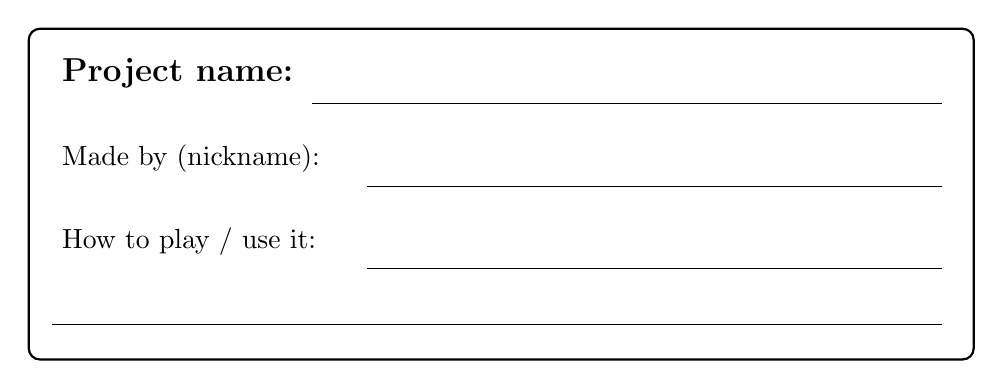
\begin{tikzpicture}
  \draw[thick, rounded corners=4pt] (0,0) rectangle (12,4.2);
  \node[anchor=north west, font=\bfseries\large] at (0.3,3.95) {Project name:};
  \draw (3.6,3.25) -- (11.6,3.25);
  \node[anchor=north west] at (0.3,2.85) {Made by (nickname):};
  \draw (4.3,2.2) -- (11.6,2.2);
  \node[anchor=north west] at (0.3,1.8) {How to play / use it:};
  \draw (4.3,1.15) -- (11.6,1.15);
  \draw (0.3,0.45) -- (11.6,0.45);
\end{tikzpicture}
\end{center}

\subsection{7.4 Feedback cards (print and cut, two per visitor)}
\begin{center}
\begin{tikzpicture}
  \foreach \x in {0,6.2} {
    \draw[thick, rounded corners=4pt] (\x,0) rectangle ++(5.9,4.4);
    \node[anchor=north west, font=\bfseries] at (\x+0.2,4.2) {Feedback for:};
    \draw (\x+2.6,3.65) -- (\x+5.6,3.65);
    \node[anchor=north west] at (\x+0.2,3.3) {\faStar\ I liked\ldots};
    \draw (\x+0.3,2.55) -- (\x+5.6,2.55);
    \node[anchor=north west] at (\x+0.2,2.2) {\faStar\ I also liked\ldots};
    \draw (\x+0.3,1.45) -- (\x+5.6,1.45);
    \node[anchor=north west] at (\x+0.2,1.1) {\faMagic\ I wish\ldots};
    \draw (\x+0.3,0.35) -- (\x+5.6,0.35);
  }
\end{tikzpicture}
\end{center}
Before visitors write, say: \enquote{Two stars and a wish: two things you liked, and one kind idea to
make it even better. Please write about the project, not the person.}

\subsection{7.5 Showcase safety}
\begin{safety}[Before the families arrive]
\begin{checklist}
  \item Every project card and every screen uses a nickname only.
  \item No program asks visitors for their real name, age, address, school or password.
  \item Nothing is uploaded or shared online. Projects stay on our Macs (copy them to a USB stick to
        keep).
  \item Photos only with the families' agreement, and only of screens and projects, not faces or name cards.
  \item Every child has credited any art, idea or code they borrowed (in a comment, and aloud if asked).
  \item A child who prefers not to present aloud may show the project one-to-one instead.
\end{checklist}
\end{safety}

\subsection{7.6 After the showcase}
Copy every project folder to a USB stick (or your own computer). Level 3 begins by putting the
children's own code under version control with git, so their Level 2 project is the perfect starting
point. Fill in the week-12 column of the progress tracker and write one specific sentence on each
certificate.

\end{document}
